\documentclass{standalone}
\usepackage{graphicx}	
\usepackage{amssymb, amsmath, amsthm}
\usepackage{color}

\usepackage{tikz}
\usetikzlibrary{math, calc, arrows.meta}

\definecolor{light}{RGB}{220, 188, 188}
\definecolor{mid}{RGB}{185, 124, 124}
\definecolor{dark}{RGB}{143, 39, 39}
\definecolor{highlight}{RGB}{180, 31, 180}
\definecolor{gray10}{gray}{0.1}
\definecolor{gray20}{gray}{0.2}
\definecolor{gray30}{gray}{0.3}
\definecolor{gray40}{gray}{0.4}
\definecolor{gray60}{gray}{0.6}
\definecolor{gray70}{gray}{0.7}
\definecolor{gray80}{gray}{0.8}
\definecolor{gray90}{gray}{0.9}
\definecolor{gray95}{gray}{0.95}

% #1: x0
% #2: y0
% #3: R
\newcommand{\randpoints}[3]{
  ({#1 + (1 + 0.2 * rand) * #3 * (-1)},      {#2 + (1 + 0.2 * rand) * #3 * (0)})
  ({#1 + (1 + 0.2 * rand) * #3 * (-0.7071)}, {#2 + (1 + 0.2 * rand) * #3 * (+0.7071)})
  ({#1 + (1 + 0.2 * rand) * #3 * (0)},       {#2 + (1 + 0.2 * rand) * #3 * (+1)})
  ({#1 + (1 + 0.2 * rand) * #3 * (+0.7071)}, {#2 + (1 + 0.2 * rand) * #3 * (+0.7071)})
  ({#1 + (1 + 0.2 * rand) * #3 * (+1)},      {#2 + (1 + 0.2 * rand) * #3 * (0)})
  ({#1 + (1 + 0.2 * rand) * #3 * (+0.7071)}, {#2 + (1 + 0.2 * rand) * #3 * (-0.7071)})
  ({#1 + (1 + 0.2 * rand) * #3 * (0)},       {#2 + (1 + 0.2 * rand) * #3 * (-1)})
  ({#1 + (1 + 0.2 * rand) * #3 * (-0.7071)}, {#2 + (1 + 0.2 * rand) * #3 * (-0.7071)})
}

\begin{document}

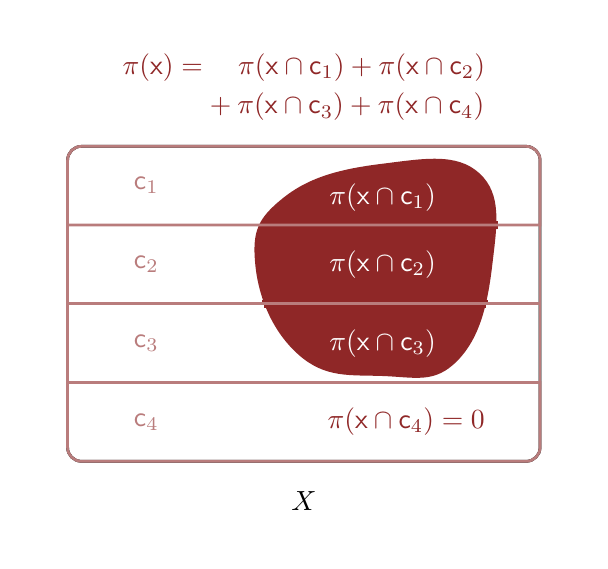
\begin{tikzpicture}[scale=1]
  \draw[white] (-0.5, -1) rectangle (6.5, 5.5);
  
  \draw[rounded corners=5, color=black, line width=1] (0, 0) rectangle (6, 4);
  \node at (3, -0.5) { $X$ };
  
  \node[dark] at (3, 5.0) { $\pi(\mathsf{x}) = \quad \pi(\mathsf{x} \cap \mathsf{c}_{1}) + \pi(\mathsf{x} \cap \mathsf{c}_{2})$ }; 
  \node[dark] at (3, 4.5) { $\hphantom{\pi(\mathsf{x}) = } + \pi(\mathsf{x} \cap \mathsf{c}_{3}) + \pi(\mathsf{x} \cap \mathsf{c}_{4})$ };
  
  \pgfmathsetseed{2}
  \fill[dark, line width=1] 
    plot [smooth cycle, tension=0.75] coordinates { \randpoints{4}{2.5}{1.5} } -- cycle;
  
  \draw[dark, line width=1] (2.45, 3.03) -- (5.46, 3.03);
  \node[white] at (4, 3.35) { $\pi(\mathsf{x} \cap \mathsf{c}_{1})$ };
  
  \draw[dark, line width=1] (2.425, 2.97) -- (5.46, 2.97);
  \draw[dark, line width=1] (2.475, 2.03) -- (5.333, 2.03);
  \node[white] at (4, 2.5) { $\pi(\mathsf{x} \cap \mathsf{c}_{2})$ };

  \draw[dark, line width=1] (2.497, 1.97) -- (5.31, 1.97);
  \node[white] at (4, 1.5) { $\pi(\mathsf{x} \cap \mathsf{c}_{3})$ };

  \node[dark] at (4.3, 0.5) { $\pi(\mathsf{x} \cap \mathsf{c}_{4}) = 0$ };
  
  \draw[mid, line width=1]
    (0, 3) -- (6, 3) {[rounded corners=5] -- (6, 4) -- (0, 4)} -- cycle;
  \node[mid] at (1, 3.5) { $\mathsf{c}_{1}$ };

  \draw[mid, line width=1]
    (0, 2) -- (6, 2) -- (6, 3) -- (0, 3) -- cycle;
  \node[mid] at (1, 2.5) { $\mathsf{c}_{2}$ };
  
  \draw[mid, line width=1]
    (0, 1) -- (6, 1) -- (6, 2) -- (0, 2) -- cycle;
  \node[mid] at (1, 1.5) { $\mathsf{c}_{3}$ };
        
  \draw[mid, line width=1]
    (0, 1) -- (6, 1) {[rounded corners=5] -- (6, 0) -- (0, 0)} -- cycle;
  \node[mid] at (1, 0.5) { $\mathsf{c}_{4}$ };

\end{tikzpicture}

\end{document}  